\documentclass[10pt,a4paper]{article}
\usepackage{amsmath,amssymb,amsthm,graphicx}
\newcommand{\RRef}{\operatorname{RRef}}
\renewcommand{\Ref}{\operatorname{Ref}}
\newcommand{\Br}{\operatorname{Br}}
\newcommand{\height}{\mathfrak h}
\newcommand{\bits}{\{0,1\}}
\newenvironment{originalresult}[1]{\par\medskip\noindent\textbf{#1.}\itshape}{\par\medskip}
\title{Depth-d Frege systems are not automatable unless P equals NP}
\author{Theodoros Papamakarios}
\date{doi:10.4230/LIPIcs.CCC.2024.22; CC BY4.0}
\begin{document}
\maketitle
\noindent\textit{Editorial note.} Faithful editable TeX transcription of the official CC BY4.0 complete published paper. Main theorem is author1.1 restated6.1, retaining P not equal NP and positive bounded depth. Complete author Sections2,3,4,5,6 proof-bearing material is included; the introductory alternative gap statement2.4 is not needed because its precise upper and lower bounds are retained as Proposition4.1 and Theorem5.5. Original Figure1 appears only as a cropped original diagram; mathematical body and LK rule table are editable. Author notation and apparent typographical choices are preserved without repair. This concerns refutation of depth-d premises as in the original paper, with no extension to a stronger CNF-only claim.\par\medskip
\noindent\textit{Allowed standard prerequisites (editorial).}\begin{itemize}
\item Bounded-depth LK and tree-like LK polynomial simulations. Source Propositions2.1/2.2, Krajicek1994 and Beckmann/Buss2005; exact statements retained
\item Resolution index-width lower bound for Ref(F,s). Source Theorem5.1, Atserias/Muller2020; exact n,s and unsatisfiability conditions retained
\item Chernoff bounds and NP completeness of3-SAT. Exact author uses retained; no recursive proof of standard background
\end{itemize}\medskip
\section*{2 Bounded-depth Frege systems and automatability (author source pp.22:3--22:5)}
\subsection*{2.1 Basic definitions}
We assume that formulas are built from constants 0 and 1, propositional variables and their negations, unbounded conjunctions and unbounded disjunctions. So negations can only appear next to variables. The depth of a formula is the maximum nesting of conjunctions and disjunctions in it. Formally,
\[d(0)=d(1)=d(x)=d(\neg x)=0,\qquad d(\circ\{F_1,\ldots,F_k\})=1+\max_i d(F_i),\]
where $x$ is a variable and $\circ$ is either a conjunction $\bigwedge$ or a disjunction $\bigvee$.
Depth-0 formulas that are not constants are called literals. We often write literals in the form $x^\varepsilon$, where $x^1:=x$ and $x^0:=\neg x$. Depth-1 formulas are called clauses/terms, clauses being disjunctions and terms conjunctions of literals. Depth-2 formulas that are disjunctions of terms are called DNF formulas and depth-2 formulas that are conjunctions of clauses are called CNF formulas. DNF formulas each conjunction of which consists of at most $k$ literals are called $k$-DNF formulas; $k$-CNF formulas are defined similarly. We define $\Sigma_d^{s,k}$ to be the class of all formulas $F$ for which there is a depth-$d$ formula $G$ that is semantically equivalent to $F$, the outermost connective of $G$ is $\bigvee$, and
\begin{enumerate}\item $G$ contains at most $s$ subformulas of depth at least 2;\item all depth-2 subformulas of $G$ are either $k$-DNFs or $k$-CNFs.\end{enumerate}
Similarly, $\Pi_d^{s,k}$ is defined as the class of all formulas $F$ for which there is a depth-$d$ formula $G$ semantically equivalent to $F$, the outermost connective of which is $\bigwedge$, satisfying the above two conditions.
A restriction is an assignment $\rho:V\to\bits$ of truth values to a set $V$ of variables. For a restriction $\rho$ and a formula $F$, we denote by $F|_\rho$ the formula resulting by replacing every variable $x$ of $F$ which is in the domain of $\rho$ by $\rho(x)$, and then eliminating constants from $F|_\rho$ using the identities
\[A\vee0=A,\quad A\vee1=1,\quad A\wedge0=0,\quad A\wedge1=A.\]
We call a restriction that gives a value to all variables a total assignment, or simply assignment. For a set $S$ of formulas, we write $S\models F$ if for any total assignment $\alpha$, $G|_\alpha=1$ for every $G\in S$ implies $F|_\alpha=1$. For formulas $F$ and $G$, we write $F\equiv G$ if $F$ and $G$ are semantically equivalent, i.e. it holds that $F\models G$ and $G\models F$.
\subsection*{2.2 LK proofs}
Bounded-depth Frege systems are commonly presented as subsystems of sequent calculus (LK for short) for propositional logic. We give a Tait-style formulation of LK, where we write cedents as disjunctions. The inference rules of the system are shown in Table1. There, $x$ stands for a propositional variable, $A$ and $B$ stand for arbitrary formulas whose top-most connective is $\bigvee$, $\varphi$ stands for an arbitrary propositional formula and $\Phi$ stands for a set of propositional formulas. $\bar\varphi$ is the formula that results from $\varphi$ by exchanging every occurrence of $\bigvee$ with $\bigwedge$ and vice versa, and replacing each literal $x^\varepsilon$ with $x^{1-\varepsilon}$.
\begin{center}\textbf{Table1: The rules of LK.}\par\medskip
$\begin{array}{r@{\quad}c} \text{Axioms:}&x\vee\neg x\\[8pt]\text{Weakening:}&\dfrac{A}{A\vee B}\\[12pt]\bigvee\text{-introduction:}&\dfrac{A\vee\varphi}{A\vee\bigvee\Phi},\quad\text{where }\varphi\in\Phi\\[12pt]\bigwedge\text{-introduction:}&\dfrac{A\vee\varphi_1\quad\cdots\quad A\vee\varphi_k}{A\vee\bigwedge\{\varphi_1,\ldots,\varphi_k\}}\\[12pt]\text{Cut:}&\dfrac{A\vee\varphi\quad B\vee\bar\varphi}{A\vee B}\end{array}$\end{center}
An LK proof from a set of premises $S$ is a sequence of formulas, called the lines of the proof, such that each line either belongs to $S$ or results from earlier lines by one of rules of Table1. If the last line in a proof is the empty disjunction, then the proof is called a refutation. A depth-$d$ LK proof is an LK proof each line of which is a formula of depth at most $d$. The size of a proof is the total number of symbols occurring in it.
Of particular importance among depth-$d$ LK proofs is the case of depth-1 proofs, called resolution proofs. In resolution proofs, lines are clauses, and the only applicable LK rules are the weakening and cut rule, which take the form
\[\frac C{C\vee D},\qquad\frac{C\vee x\quad D\vee\neg x}{C\vee D}\]
for clauses $C$ and $D$. In the rightmost rule, also called the resolution rule, we say that $C\vee D$ is the result of resolving $C\vee x$ on $D\vee\neg x$ on $x$.
We may view a proof as a DAG, by drawing for every line $A$, edges from the lines $A$ is derived to $A$. In case a proof DAG is a tree, we refer to the proof as being tree-like. The next propositions, due to[14], state that depth-$d$ LK proofs and tree-like depth-$(d+1)$ LK proofs can be turned into one another with only a polynomial increase in size.
\begin{originalresult}{Proposition 2.1 [14]}
A depth-$d$ LK proof of a formula $F$ from $S$ of size $s$ can be turned into a depth-$(d+1)$ tree-like LK proof of $F$ from $S$ of size polynomial in $s$.
\end{originalresult}
\begin{originalresult}{Proposition 2.2 [14,3]}
Let $S$ be a set of formulas of depth at most $d$ and $F$ a formula of depth at most $d$. A depth-$(d+1)$ tree-like LK proof of a formula $F$ from $S$ of size $s$ can be turned into a depth-$d$ LK proof of $F$ from $S$ of size $O(s^2)$.
\end{originalresult}
\subsection*{2.3 Semantic proofs, variable width and decision trees}
A semantic depth-$d$ (Frege) proof from a set of formulas $S$ is a sequence of depth-$d$ formulas $F_1,\ldots,F_t$ such that for every $i$, either $F_i\in S$ or there are $j,k<i$ such that $F_j,F_k\models F_i$. Notice that if $S$ consists of depth-$(d-1)$ formulas, then there is a trivial depth-$d$ proof of any valid consequence of $S$, as $\bigwedge S$ can be derived in $|S|-1$ steps. Thus, under this formulation, depth-$d$ proofs from $S$ are interesting only if $S$ contains depth-$d$ formulas not in $\Pi_d^{s,k}$ for any $s$ and $k$, and indeed, our results pertain to such proofs.
The definitions of lines, size of a proof, refutation, tree-like proofs, apply to semantic proofs as well. The variable width of a proof is the maximum number of variables among the lines of the proof.
Unlike size, variable width is an inherently semantic notion. In particular, it is independent of depth: any depth-$d$ proof of variable width $w$ can be transformed into a depth-1 proof of (variable) width $O(w)$. In fact, something stronger can be said. A decision tree is a binary tree the internal nodes of which are labelled by variables, and the edges by values 0 or1. Nodes query variables and the edges going from a node to its children are labelled, one by the value0 and the other by1, giving an answer to that query. No variable is repeated in a branch so that branches correspond to restrictions, and each branch has a value,0 or1, associated with it, so that the decision tree represents a Boolean function. We denote the set of branches of $T$ having the value $v$ by $\Br_v(T)$. Specifically, we say that a decision tree $T$ represents a formula $F$ if for every branch $\pi$ of $T$ with value $v$, $F|_\pi\equiv v$. The height of a decision tree is the length of its longest branch. Notice that if a formula $F$ is represented by a decision tree of height $h$, then $F\in\Sigma_2^{1,h}\cap\Pi_2^{1,h}$. We write $\height(F)$ for the minimum height of a decision tree representing $F$. The following lemma is shown in[18] for a specific type of depth-2 proofs, but holds for proofs of arbitrary depth, or for that matter, arbitrary sound proofs.
\begin{originalresult}{Lemma 2.3}
Let $S$ be a set of clauses each containing at most $h$ literals. If there is a semantic refutation of $S$ each line of which is represented by a decision tree of height at most $h$, then there is a resolution refutation of $S$ of width at most $3h$.
\end{originalresult}
\begin{proof}
Let $F_1,\ldots,F_t$ be a semantic refutation of $S$ and let $T_i$ be a decision tree of height at most $h$ representing $F_i$. We assume that $T_t$ has a single node having the value0. For a restriction $\pi$, let $C_\pi$ be the minimal clause falsified by $\pi$. We will show that for every $i$, for every branch $\pi\in\Br_0(T_i)$, we can derive $C_\pi$ via a resolution proof of width at most $3h$. Notice that $C_\pi$ for $\pi\in\Br_0(T_t)$ is the empty clause, so this construction will give a refutation.
If $F_i$ is a clause $C$ in $S$, then every $\pi\in\Br_0(T_i)$ must make every literal in $C$ false, hence $C_\pi$ is a weakening of $C$. Assume now that $F_i$ is derived from $F_j$ and $F_k$ and we have derived all clauses $C_\pi$ for $\pi\in\Br_0(T_j)\cup\Br_0(T_k)$. Let $\sigma\in\Br_0(T_i)$, and let $T$ be the tree resulting by appending a copy of $T_k$ at the end of every branch $\pi\in\Br_1(T_j)$ of $T_j$. We will use $T$ to extract a resolution proof of $C_\sigma$. More specifically, for every node $u$ of $T$ such that the path $\pi_u$ from the root of $T$ to $u$ corresponds to a restriction that is consistent with $\sigma$, we will derive $C_\sigma\vee C_{\pi_v}$. When we reach the root of $T$ we will have derived $C_\sigma$. If $u$ is a leaf of $T$, then we claim that $C_{\pi_u}$ is a weakening of some clause $C_\pi$ for $\pi\in\Br_0(T_j)\cup\Br_0(T_k)$. To see this, let $\pi_u=\pi_j\cup\pi_k$, where $\pi_j$ is the part of $\pi_u$ that belongs to $T_j$ and $\pi_k$ the part that belongs to $T_k$. Since $F_j,F_k\models F_i$ and $\pi_u$ is consistent with $\sigma$, it cannot be the case that both $\pi_j\in\Br_1(T_j)$ and $\pi_k\in\Br_1(T_k)$, otherwise a total assignment extending both $\pi_u$ and $\sigma$ would make $F_j$ and $F_k$ true, but $F_i$ false. Suppose now that $u$ is not a leaf of $T$ and suppose that $v$ and $w$ are its children. Then either $\pi_v$ and $\pi_w$ are both consistent with $\sigma$, in which case $C_\sigma\vee C_{\pi_u}$ can be derived by resolving $C_\sigma\vee C_{\pi_v}$ and $C_\sigma\vee C_{\pi_w}$ on the variable labelling $u$, or one of the children, say $v$, will be consistent with $\sigma$ and thus $C_\sigma\vee C_{\pi_u}$ will be identical to $C_\sigma\vee C_{\pi_v}$.
\end{proof}
\subsection*{2.4 Automatability and the main result}
A proof system $\sigma$ is called automatable[5] if there is an algorithm that given a set of formulas $S$ and a formula $\varphi$ provable from $S$, outputs a $\sigma$-proof of $\varphi$ from $S$ in time polynomial $r+s$, where $r$ is the total size of $S$ and $s$ the size of the shortest $\sigma$-proof of $\varphi$ from $S$.

\section*{3 The formulas Ref (author source pp.22:6--22:8)}
Let $F$ be a CNF formula with $n$ variables and $m$ clauses. The key ingredient in the non-automatability result of[2] is expressing by a set of clauses $\Ref(F,s)$ the statement that there is a resolution refutation $D_1,\ldots,D_s$ of length $s$ from the clauses of $F$.
The variables of $\Ref(F,s)$ are $D[u,i,b],V[u,i],I[u,j],L[u,v]$ and $R[u,v]$, where $u,v\in[s],i\in[n],j\in[m]$ and $b\in\bits$. The meaning of $D[u,i,b]$ is that $x_i^b$ appears in $D_u$. The meaning of $V[u,i]$ is that $D_u$ is derived as a weakening of the resolvent of two previous clauses on $x_i$, and the meaning of $I[u,j]$ is that $D_u$ is a weakening of the $j$-th clause of $F$. The meaning of $L[u,v]$ is that the left clause (i.e. that which contains $\neg x_i$) from which $D_u$ was derived is $D_v$, and the meaning of $R[u,w]$ is that the right clause (i.e. that which contains $x_i$) from which $D_u$ was derived is $D_w$. We will also use the variables $V[u,0]$ and $I[u,0]$ to indicate whether $D_u$ is derived from previous clauses or from an initial clause of $F$: in the former case,$I[u,0]$ will be true and $V[u,0]$ false, and in the latter $V[u,0]$ will be true and $I[u,0]$ false. The clauses of $\Ref(F,s)$ encode the following conditions: For each $u,v\in[s],i,i'\in[n],j\in[m]$ and $b\in\bits$,
\begin{align*}
&\exists!k\ V[u,k]\ \&\ \exists!k\ I[u,k]\ \&\ \exists!k\ L[u,k]\ \&\ \exists!k\ R[u,k];\tag{3.1}\\
&V[u,0]\iff\neg I[u,0];\tag{3.2}\\
&\neg L[u,v]\text{ for }v\ge u\ \&\ \neg R[u,v]\text{ for }v\ge u;\tag{3.3}\\
&V[u,i]\ \&\ L[u,v]\implies D[v,i,0];\tag{3.4}\\
&V[u,i]\ \&\ R[u,v]\implies D[v,i,1];\tag{3.5}\\
&V[u,i]\ \&\ L[u,v]\ \&\ D[v,i',b]\ \&\ i\ne i'\implies D[u,i',b];\tag{3.6}\\
&V[u,i]\ \&\ R[u,v]\ \&\ D[v,i',b]\ \&\ i\ne i'\implies D[u,i',b];\tag{3.7}\\
&I[u,j]\ \&\ x_i^b\text{ appears in }C_j\implies D[u,i,b];\tag{3.8}\\
&\neg D[u,i,0]\vee\neg D[u,i,1];\tag{3.9}\\
&\neg D[s,i,b].\tag{3.10}
\end{align*}
It was shown, subsequent to[2], that $\Ref(F,s)$ is hard for resolution whenever $F$ is unsatisfiable[9]. In[2], a variation,$\RRef(F,s)$, is used. $\RRef(F,s)$ expresses the fact that there is a resolution refutation $D_1,\ldots,D_s$ or one contained in $D_1,\ldots,D_s$, from the clauses of $F$. $\RRef(F,s)$ has the same variables as $\Ref(F,s)$ plus a new variable $P[u]$ indicating which of the indices $1,\ldots,s$ are active, i.e. are part of the refutation. The clauses of $\RRef(F,s)$ express the following conditions, which are those of $\Ref(F,s)$ conditioned on the fact that $P[u]$ is true, in addition to three new ones requiring $P[s]$ to be true, and $P[v]$ to be true whenever $P[u]$ and $L[u,v]$ or $R[u,v]$ are true:
\begin{align*}
&P[u]\implies\exists!k\ V[u,k]\ \&\ \exists!k\ I[u,k]\ \&\ \exists!k\ L[u,k]\ \&\ \exists!k\ R[u,k];\tag{3.11}\\
&P[u]\implies(V[u,0]\iff\neg I[u,0]);\tag{3.12}\\
&P[u]\implies\neg L[u,v]\text{ for }v\ge u\ \&\ \neg R[u,v]\text{ for }v\ge u;\tag{3.13}\\
&P[u]\implies(V[u,i]\ \&\ L[u,v]\implies D[v,i,0]);\tag{3.14}\\
&P[u]\implies(V[u,i]\ \&\ R[u,v]\implies D[v,i,1]);\tag{3.15}\\
&P[u]\implies(V[u,i]\ \&\ L[u,v]\ \&\ D[v,i',b]\ \&\ i\ne i'\implies D[u,i',b]);\tag{3.16}\\
&P[u]\implies(V[u,i]\ \&\ R[u,v]\ \&\ D[v,i',b]\ \&\ i\ne i'\implies D[u,i',b]);\tag{3.17}\\
&P[u]\implies(I[u,j]\ \&\ x_i^b\text{ appears in }C_j\implies D[u,i,b]);\tag{3.18}\\
&P[u]\implies(\neg D[u,i,0]\vee\neg D[u,i,1]);\tag{3.19}\\
&P[s]\ \&\ \neg D[s,i,b];\tag{3.20}\\
&(P[u]\ \&\ L[u,v]\implies P[v])\ \&\ (P[u]\ \&\ R[u,v]\implies P[v]).\tag{3.21}
\end{align*}
Notice that giving truth values to the $P[u]$ variables (where $P[s]=1$) reduces $\RRef(F,s)$ to $\Ref(F,s')$ where $s'$ is the number of indices $u$ for which $P[u]=1$.
For an integer $k\ge1$, we define $R^k\Ref(F,s)$ as the formula resulting from substituting each variable $P[u]$ in $\RRef(F,s)$ with the conjunction $\bigwedge_{i=1}^kP_i[u]$ for new variables $P_1[u],\ldots,P_k[u]$. Note that $\RRef(F,s)=R^1\Ref(F,s)$.
Now, let $d,N\ge1$ be integers, and let $x$ be a propositional variable. We associate with $x$ $N^{d-1}\lceil\sqrt N/2\rceil$ new variables $x_{i_1,\ldots,i_d}$, where $i_1,\ldots,i_{d-1}\in[N]$ and $i_d\in[\lceil\sqrt N/2\rceil]$. The fact that we make $i_d$ range over $[\lceil\sqrt N/2\rceil]$ instead of $[N]$ will be important later (specifically in Lemma5.2). The depth-$d$ Sipser functions for $x$ are defined by
\begin{align*}
S_{d,N}^{\wedge}(x)&\stackrel{\rm def}=\bigwedge_{i_1=1}^N\bigvee_{i_2=1}^N\cdots\bigwedge_{i_d=1}^{\lceil\sqrt N/2\rceil}x_{i_1,\ldots,i_d},\\
S_{d,N}^{\vee}(x)&\stackrel{\rm def}=\bigvee_{i_1=1}^N\bigwedge_{i_2=1}^N\cdots\bigvee_{i_d=1}^{\lceil\sqrt N/2\rceil}x_{i_1,\ldots,i_d}
\end{align*}
if $d$ is odd, and
\begin{align*}
S_{d,N}^{\wedge}(x)&\stackrel{\rm def}=\bigwedge_{i_1=1}^N\bigvee_{i_2=1}^N\cdots\bigvee_{i_d=1}^{\lceil\sqrt N/2\rceil}x_{i_1,\ldots,i_d},\\
S_{d,N}^{\vee}(x)&\stackrel{\rm def}=\bigvee_{i_1=1}^N\bigwedge_{i_2=1}^N\cdots\bigwedge_{i_d=1}^{\lceil\sqrt N/2\rceil}x_{i_1,\ldots,i_d}
\end{align*}
if $d$ is even.
We define $\RRef_{d,N}(F,s)$ to be the result of substituting every variable of the form $P[u]$ in $\RRef(F,s)$ with $S_{d,N}^{\wedge}(P[u])$ and every other variable $x$ with $S_{d,N}^{\vee}(x)$. Notice that $\RRef_{d,N}(F,s)$ is a set of depth-$(d+1)$ formulas. But, as we want to prove statements about whether $\RRef_{d,N}(F,s)$ has or does not have small depth-$d$ refutations, we must write it as a set of depth-$d$ formulas. We may do that with only a polynomial increase in size, as the only clauses of non constant size of $\RRef(F,s)$ are those of the form $\neg P[u]\vee\bigvee_i X[u,i]$ corresponding to conditions(3.11), and these clauses will have depth-$d$ after the substitution taking us from $\RRef(F,s)$ to $\RRef_{d,N}(F,s)$. Note that the conversion from $\RRef_{d,N}(F,s)$ written as a set of depth-$d$ formulas to its equivalent set of depth-$(d+1)$ formulas can be carried in tree-like depth-$(d+1)$ LK in linear time. In particular, a tree-like depth-$(d+1)$ LK refutation of the latter set can be turned into a tree-like depth-$(d+1)$ LK refutation of the former set, increasing the size by at most a factor of $N^3$.

\section*{4 Upper bounds (author source pp.22:8--22:10)}
We show in this section that if $F$ is satisfiable, then $\RRef_{d,N}(F,s)$ has small depth-$d$ refutations:
\begin{originalresult}{Proposition 4.1}
If $F$ is a satisfiable CNF formula with $n$ variables and $m$ clauses, then there is a depth-$d$ LK refutation of $\RRef_{d,N}(F,s)$ of size
\[S=O\left(\left(N^{d+3}s^2n(m+s^2n^3)\right)^2\right).\]
In particular, if $m=O(s^2n^3)$, then $S=O(N^{2(d+3)}(sn)^8)$.
\end{originalresult}
\begin{proof}
We start with a small depth-2 LK tree-like refutation of $\RRef(F,s)$. This refutation will be such that after the substitution with Sipser functions, we get a depth-$(d+1)$ tree-like refutation of $\RRef_{d,N}(F,s)$, which in turn we can convert to a depth-$d$ DAG-like refutation of $\RRef_{d,N}(F,s)$ by Proposition2.2.
We write, for better readability, $A_1,\ldots,A_k\to B_1,\ldots,B_\ell$ instead of $\bar A_1\vee\cdots\vee\bar A_k\vee B_1\vee\cdots\vee B_\ell$.
Let $\alpha$ be an assignment that satisfies every clause of $F$. We set
\[T(u):=P[u]\to\bigvee_{i=1}^n D[u,i,\alpha(x_i)].\]
What $T(u)$ says is that if $P[u]$ is true, then $\alpha$ satisfies the $u$-th clause in the refutation $\Ref(F,s)$ describes.
Our refutation of $\RRef(F,s)$ consists of $s-1$ stages, starting with stage0. In the $u$-th stage, $T(1),\ldots,T(s-u)\to0$ will have been derived. Then we can use this formula, along with a derivation of $T(1),\ldots,T(s-u-1)\to T(s-u)$, to derive $T(1),\ldots,T(s-u-1)\to0$. In the $s-1$-th stage, $T(1)\to0$ will have been derived, at which point we can reach a contradiction by deriving $T(1)$.
A derivation of $T(1),\ldots,T(v-1)\to T(v)$ is sketched in Figure1.
\begin{figure}[ht]\centering\includegraphics[page=9,width=.82\textwidth,trim=90 400 100 210,clip]{frege-original.pdf}\caption{Original Figure1: A sketch of a derivation of $T(1),\ldots,T(v-1)\to T(v)$.}\end{figure}
The formulas $I[v,j]\to T(v)$ for $j\in[m]$ can be immediately derived from the clauses $P[u]\wedge I[v,j]\to D[v,i,\alpha(x_i)]$, which are clauses corresponding to condition(3.18), as the fact that $\alpha$ satisfies the clause $C_j$ means that $x_i^{\alpha(x_i)}$ must belong to $C_j$ for some $i$. These formulas can be in turn used along with the clauses(3.11) for $I[v,k]$ and(3.12) to derive $V[v,0]\to T(v)$. Now deriving
\[T(1),\ldots,T(v-1)\to V[v,0],T(v)\tag{4.1}\]
will allow us to derive $T(1),\ldots,T(v-1)\to T(v)$ by cutting on $V[v,0]$. We can derive(4.1) from the formulas
\[T(1),\ldots,T(v-1),V[v,i]\to T(v)\tag{4.2}\]
for $i\in[n]$ using the clauses(3.11) for $V[v,i]$. The formulas(4.2) can be in turn derived from the formulas
\[T(v_\ell),L[v,v_\ell],T(v_r),R[u,v_r],V[v,i]\to T(v)\tag{4.3}\]
for $v_\ell,v_r\in[s]$ using the clauses(3.11) for $L[v,k]$ and $R[v,k]$,(3.12) and(3.13). Finally,(4.3) can be derived from the formulas
\[D[v_\ell,j,\alpha(x_j),L[v,v_\ell],D[v_r,x_k,\alpha(x_k)],R[u,v_r],V[v,i]\to T(v),\tag{4.4}\]
for $j,k\in[n]$, which can be derived directly from the clauses(3.21) and either(3.14),(3.15) and(3.19) or(3.16) and(3.17) depending on whether $i=j=k$ or not.
We can see that the derivations of $T(1),\overline{T(s)}$ and $T(1),\ldots,T(v-1)\to T(v)$ take at most $O(m+s^2n^3)$ steps, hence the overall refutation has size $O(s^2n(m+s^2n^3))$.
Now, notice that after substituting every variable $P[u]$ in it with $S_{d,N}^{\wedge}(P[u])$ and every other variable $x$ with $S_{d,N}^{\vee}(x)$, $T(v)$ becomes a depth-$d$ formula. Hence we see that after the substitution, the refutation described above becomes a depth-$(d+1)$ tree-like LK refutation of $\RRef_{d,N}(F,s)$. We can then get a depth-$d$ refutation of $\RRef_{d,N}(F,s)$ of the required size by applying Proposition2.2.
\end{proof}

\section*{5 Lower bounds (author source pp.22:10--22:12)}
Lower bounds for depth-$d$ Frege systems for $d>1$, typically follow the following strategy:
\begin{enumerate}\item We first show that the formulas we are trying to refute are robust; namely, after applying a restriction selected at random to them, then with high probability they cannot be refuted with proofs whose lines are, in a certain sense, simple.\item Then we show, through the use of a switching lemma, that applying such a restriction to a short proof will result with high probability in a proof with simple lines.\end{enumerate}
Here we start with $\RRef_{d,N}(F,s)$, which after applying the restrictions will collapse to $\Ref(F,s')$, where $s'$ is polynomially related to $s$. For the part of the overall strategy showing that there cannot be refutations with simple lines, we take, as in[2], simple to mean of small index-width. We say that a variable of the form $D[u,i,b],V[u,i],I[u,j],L[u,v]$ or $R[u,v]$ mentions the index $u$. The index-width of a clause in the variables of $\Ref(F,s)$ is defined as the number of indices mentioned by its variables, and the index-width of a resolution refutation of $\Ref(F,s)$ is the maximum index-width over its clauses. We have:
\begin{originalresult}{Theorem 5.1 [2]}
For all integers $n,s>0$ with $s\le2^n$, and every unsatisfiable CNF $F$ with $n$ variables, every resolution refutation of $\Ref(F,s)$ has index-width at least $s/6n$.
\end{originalresult}
\subsection*{5.1 The robustness of $\RRef_{d,N}$}
We create a distribution on restrictions to the variables of $\RRef_{d,N}(F,s)$ as follows. Suppose $d$ is odd (if $d$ were even, we would exchange the roles of0 and1 in the following construction). For each $S_{d,N}^{\wedge}(x)$ formula in $\RRef_{d,N}(F,s)$, look at its bottom-most $N^{d-1}$ $\bigwedge$ connectives. For each such connective, we decide to ``preserve'' it with probability $1/\sqrt N$, and not to preserve it with probability $1-1/\sqrt N$. For each of the preserved connectives, we leave its first variable unset and set the rest to1. For each variable in the unpreserved connectives, we set it to0 or1 with probability $1/2$ for each choice. The variables of $S_{d,N}^{\vee}(x)$ are set in the same way, except that the set variables of the preserved $\bigvee$ connectives are set to0 instead of1.
Under such restrictions, Sipser functions do not simplify much. For formulas $F$ and $G$, in which each variable appears only once, we say that $F$ contains $G$ if we can get $G$ from $F$ by deleting some of its literals and/or renaming some of its variables.
\begin{originalresult}{Lemma 5.2}
For any $d\ge2$, the probability that $S_{d,N}^{\nu}(x)|_\rho$, where $\nu\in\{\wedge,\vee\}$, does not contain $S_{d-1,N}^{\nu}(x)$ is at most $2^{-\Omega(\sqrt N)}$.
\end{originalresult}
\begin{proof}
We show the lemma for $S_{d,N}^{\wedge}(x)$ and $d$ odd. If $S_{d,N}^{\wedge}(x)|_\rho$ does not contain $S_{d-1,N}^{\wedge}$, then either one of its bottom-most $\bigwedge$ connectives takes the value1, or in one of its depth-2 subformulas, less than $\sqrt N/2$ $\bigwedge$ connectives are preserved. The probability that a bottom-most $\bigwedge$ connective takes the value1 is at most $2^{-\sqrt N/2}$ and the probability that this happens for at least one of the $N^{d-1}$ bottom-most $\bigwedge$ connectives is at most
\[N^{d-1}2^{-\sqrt N/2}\le2^{-\Omega(\sqrt N)}.\]
Now fix a depth-2 subformula $A$ of $S_{d,N}^{\wedge}(x)$. The expected number of preserved $\bigwedge$ connectives in $A|_\rho$ is $N/\sqrt N=\sqrt N$, and by the Chernoff bound, the probability that there are less than $\sqrt N/2$ preserved $\bigwedge$ connectives is at most $2^{-\Omega(\sqrt N)}$. The probability that at least one of the $N^{d-2}$ depth-2 subformulas of $S_{d,N}^{\wedge}(x)$ has less than $\sqrt N/2$ preserved connectives is thus at most
\[N^{d-2}2^{-\Omega(\sqrt N)}\le2^{-\Omega(\sqrt N)}.\]
We conclude that the probability that $S_{d,N}^{\wedge}|_\rho$ does not contain $S_{d-1,N}^{\wedge}$ is at most $2^{-\Omega(\sqrt N)}$.
\end{proof}
\subsection*{5.2 The Furst-Saxe-Sipser switching lemma}
Switching lemmas provide conditions under which a $k$-DNF formula ``switches'' to a $\ell$-CNF formula after applying a restriction created at random. We will use the switching lemma of[8] and a variation tailored for $R^k\Ref(F,s)$ due to[10].
Let $G$ be a $k$-DNF formula over the set of variables $X$. Let $X_1,\ldots,X_r$ be a partition of $X$ into $r$ blocks, and let $\nu\in\bits$. Consider the following distribution over restrictions on $X$: For each block $X_i$, we decide to ``preserve'' $X_i$ with probability $p$, and not to preserve it with probability $1-p$. For each preserved block, we leave one of its variables, say the first in the block, unset, and set all others to $\nu$. For each unpreserved block, we set each of its variables to0 or1 with probability $1/2$ for each value.
We can extract the following lemma from[8,19]. The lemma is implicit in[8,19] with parameters obscured under a big $O$ notation. We present it here in a more general, improved form, with explicit parameters, using decision trees along the lines of[18]. In what follows,$\ln$ denotes the natural logarithm; we preserve the notation $\log$ for the base2 logarithm.
\begin{originalresult}{Lemma 5.3 (see[8,19])}
If $phk2^k\ln N=o(N^{-\varepsilon})$ for some $\varepsilon\in(0,1)$, then
\[\mathbb P[\height(G|_\rho)>kh]\le o(N^{-\varepsilon h})\frac{2^{kh}-1}{2^h-1}.\]
\end{originalresult}
\begin{proof}
The proof is by induction on $k$. If $k=0$, $G$ is a constant and can be represented by a decision tree of height0. Suppose $k>0$. We distinguish between two cases,$G$ being wide and $G$ being narrow. We call $G$ wide if there are at least $h2^k\ln N$ terms in it such that no two of them contain variables from the same block. $G$ is narrow if and only if it is not wide. If $G$ is wide, then
\begin{align*}
\mathbb P[\height(G|_\rho)>kh]&\le\mathbb P[G|_\rho\ne1]\le\left(1-\left(\frac{1-p}{2}\right)^k\right)^{h2^k\ln N}\\
&\le e^{-(1-p)^k h\ln N}=N^{-(1-p)^kh}=o(N^{-\varepsilon h}).
\end{align*}
If $G$ is narrow, then take a maximal set of terms such that no two of them contain variables from the same block, and let $H$ be the set of blocks that contain a variable occurring in some term of this set. $H$ contains at most $hk2^k\ln N$ blocks and every term of $G$ contains some variable (or its negation) from some block in $H$. The probability of the event $A$ that $\rho$ preserves more than $h$ blocks in $H$ is
\[\mathbb P[A]\le\binom{hk2^k\ln N}{h}p^h\le(hk2^k\ln N)^hp^h=o(N^{-\varepsilon h}).\]
Now, let $\pi$ be a restriction that sets the variables of all blocks in $H$, and let $A_\pi$ be the event that $\pi$ is consistent with $\rho$ and $\height((G|_\rho)|_\pi)>(k-1)h$. Notice that $G|_\pi$ is a $(k-1)$-DNF, so by the induction hypothesis,
\[\mathbb P[A_\pi]\le\mathbb P[\height((G|_\pi)|_\rho)>(k-1)h]\le o(N^{-\varepsilon h})\frac{2^{(k-1)h}-1}{2^h-1}.\]
Notice that a restriction $\rho$ that preserves at most $h$ blocks is consistent with at most $2^h$ restrictions $\pi$, so we get
\[\mathbb P\left[A\cup\bigcup_\pi A_\pi\right]\le o(N^{-\varepsilon h})+o(N^{-\varepsilon h})2^h\frac{2^{(k-1)h}-1}{2^h-1}=o(N^{-\varepsilon h})\frac{2^{kh}-1}{2^h-1}.\]
In the event $\left(A\cup\bigcup_\pi A_\pi\right)^c$, i.e. the event that $\rho$ preserves at most $h$ blocks in $H$ and for all restrictions $\pi$ consistent with $\rho$,$\height((G|_\rho)|_\pi)\le(k-1)h$, we can construct a decision tree of height at most $kh$ representing $G|_\rho$ as follows: We query all variables belonging to some block in $H$ left unset by $\rho$ (since $\rho$ preserves at most $h$ blocks in $H$, there are at most $h$ of them), and at each branch $\pi$ of the resulting tree, we append a decision tree of minimum height representing $(G|_\rho)|_\pi$.
\end{proof}

\section*{Index restrictions and switching (author source pp.22:12--22:14)}
We create a distribution on restrictions on the variables of $R^\ell\Ref(F,s)$ as follows: For every index $u$ and every $i\in[\ell]$, we set $P_i[u]$ to0 or1, with probability $1/2$ for each value. Let $U$ be the set of indices such that $P_i[u]=1$ for all $i\in[\ell]$. For each variable $x$ of $R^\ell\Ref(F,s)$ not of the form $P_i[u]$ mentioning an index in $U$, we set $x$ to0 or1, with probability $1/2$ for each value.
For a decision tree $T$ querying variables of $\Ref(F,s)$, we define the index-height of $T$ as the maximum number of indices mentioned by variables over all branches that do not falsify axioms of $\Ref(F,s)$. For a formula $G$, We denote by $\hbar(G)$ the minimum index-height of a decision tree representing $G$.
The following lemma is from[10]. We give a proof because in[10] the lemma is stated not for $R^\ell\Ref(F,s)$ but a variation, plus we view the following proof to be simpler.
\begin{originalresult}{Lemma 5.4 [10]}
Let $F$ be a CNF formula in $n$ variables,$k$ and $\ell$ integers with $0<k\le\ell$, and $G$ a $k$-DNF formula over the variables of $R^\ell\Ref(F,s)$, where $s\le2^{\delta n}$ for some $\delta<1$. Then for large enough $n$,
\[\mathbb P[\hbar(G|_\rho)>h]\le2^{-\frac h{n^{k-1}}\gamma(k)},\]
where $\gamma(0)=1,\gamma(i)=(\log e)(i4^{i+1})^{-1}\gamma(i-1)$.
\end{originalresult}
\begin{proof}
Let $h_i:=h\gamma(i-1)/(4n^{i-1})$. We will show, by induction on $k$, that for every $k$ and $\ell$ with $k\le\ell$, for every $k$-DNF formula $G$ over the variables of $R^\ell\Ref(F,s)$,
\[\mathbb P\left[\hbar(G|_\rho)>\sum_{i=1}^kh_i\right]\le2^{-\frac h{n^{k-1}}\gamma(k)}\]
for large enough $n$.
If $k=0$, $F$ is a constant and can be represented by a decision tree of height0. Suppose $k>0$. We call $G$ wide if there are at least $h_k/k$ terms in $G$ over disjoint sets of indices, and call $G$ narrow otherwise. Suppose $G$ is wide. A literal in a term $t$ of $G$ is satisfied with probability at least $1/4$: Literals on a variable $P_i[u]$ are satisfied with probability $1/2$. For any other literal $x^\epsilon$ of $t$ mentioning the index $u$, since $k\le\ell$, there must be a variable $P_i[u]$ not in $t$, which is made0 with probability $1/2$, in which case $x^\epsilon$ will be satisfied with probability $1/2$. Hence
\begin{align*}
\mathbb P[\hbar(G|_\rho)>h]&\le\mathbb P[G|_\rho\ne1]\le(1-4^{-k})^{\frac{h\gamma(k-1)}{4kn^{k-1}}}\\
&\le2^{-\frac h{n^{k-1}}(\log e)(k4^{k+1})^{-1}\gamma(k-1)}=2^{-\frac h{n^{k-1}}\gamma(k)}.
\end{align*}
Suppose now that $G$ is narrow. Take a maximal set of terms over disjoint sets of indices, and let $H$ be the set of indices that are mentioned by the terms of this set. Notice that $|H|\le h_k$ and that every term of $G$ contains some variable (or its negation) that mentions an index in $H$. Let $\pi$ be a restriction that
\begin{enumerate}\item sets all variables mentioning an index in $H$ and leaves all other variables unset, and\item does not falsify any axioms of $R^\ell\Ref(F,s)$.\end{enumerate}
The second condition means in particular that if $U$ is the set of indices $u$ for which $\pi$ sets $P_i[u]$ to1 for all $i$, then for all $u\in U$, there will be exactly one $v$ such that $L[u,v]$ is true, exactly one $v$ such that $R[u,v]$ is true, exactly one $i$ such that $V[u,i]$ is true, and exactly one $j$ such that $I[u,j]$ is true, making the total number of such $\pi$'s to be at most
\[S^{|U|}2^{(|H|-|U|)n_0}\]
where $S:=s^2(n+1)(m+1)2^{2n}$ and $n_0$ is the number of variables of $R^\ell\Ref(F,s)$ mentioning a fixed index $u$.
Let $A_\pi$ be the event that $\pi$ is consistent with $\rho$ and $\hbar((G|_\rho)|_\pi)>\sum_{i=i}^{k-1}h_i$. We have that
\begin{align*}
\mathbb P[A_\pi]&=\mathbb P\left[\hbar((G|_\rho)|_\pi)>\sum_{i=i}^{k-1}h_i\mid\rho\text{ con.with }\pi\right]\mathbb P[\rho\text{ con.with }\pi]\\
&=\mathbb P\left[\hbar((G|_\pi)|_\rho)>\sum_{i=i}^{k-1}h_i\right]\mathbb P[\rho\text{ con.with }\pi]\\
&\le2^{-\frac h{n^{k-2}}\gamma(k-1)}2^{-\ell|U|}2^{-(|H|-|U|)n_0}.
\end{align*}
Hence, we get
\begin{align*}
\mathbb P\left[\bigcup_\pi A_\pi\right]&\le\sum_\pi\mathbb P[A_\pi]\\
&\le\sum_{U\subseteq H}S^{|U|}2^{(|H|-|U|)n_0}2^{-\frac h{n^{k-2}}\gamma(k-1)}2^{-\ell|U|}2^{-(|H|-|U|)n_0}\\
&=\sum_{r=0}^{|H|}\binom{|H|}{r}S^r2^{-\frac h{n^{k-2}}\gamma(k-1)}2^{-\ell r}\\
&=(S/2^\ell+1)^{|H|}2^{-\frac h{n^{k-2}}\gamma(k-1)}\\
&\le S^{|H|}2^{-\frac h{n^{k-2}}\gamma(k-1)}.
\end{align*}
Since $s\le2^{\delta n}$ for some $\delta<1$, the quantity
\[S^{|H|}=\left(s^2(n+1)(m+1)2^{2n}\right)^{\frac h{4n^{k-1}}\gamma(k-1)}\]
will be at most $2^{\frac{\varepsilon h}{n^{k-2}}\gamma(k-1)}$ for some $\varepsilon<1$ for large enough $n$, therefore
\[\mathbb P\left[\bigcup_\pi A_\pi\right]\le2^{-\frac h{n^{k-1}}\gamma(k)}\]
for large enough $n$.
In the event $\left(\bigcup_\pi A_\pi\right)^c$, that is the event that for every $\pi$ consistent with $\rho$, $\hbar((G|_\rho)|_\pi)\le\sum_{i=1}^{k-1}h_i$, we can construct a decision tree for $G|_\rho$ of index-height at most $\sum_{i=1}^kh_i$ as follows: We first query all variables mentioning an index in $H$ left unset by $\rho$. Then, at each branch $\pi$ of the resulting tree, we append a decision tree of minimum index-height representing $(G|_\rho)|_\pi$.
\end{proof}

\section*{5.3 The lower bound for $\RRef_{d,N}$ (author source pp.22:14--22:15)}
\begin{originalresult}{Theorem 5.5}
For every integer $d>0$, if $F$ is an unsatisfiable CNF in $n$ variables,$N$ is an increasing function of $n$ and $s$ is a polynomial in $n$, every semantic depth-$d$ refutation of $\RRef_{d,N}(F,s)$ has size at least
\[N^{\frac13\left(\frac{\log s}{\log n}-2\right)^{\frac1{d-1}}}\]
for large enough $n$.
\end{originalresult}
\begin{proof}
Let $h:=(1/3)(\log s/\log n-2)^{1/(d-1)}$ and let $G_1,\ldots,G_t$ be a semantic depth-$d$ refutation of $\RRef_{d,N}(F,s)$ of size at most $N^h$. We assume that each $G_i$ is either a literal or a disjunction of its immediate subformulas. Let $A$ be a depth-1 subformula of some $G_i$. $A$ is a1-DNF or a1-CNF formula, so applying Lemma5.3 to it (or its negation respectively) with $k=1$ and $p=N^{-1/2}$ and using as blocks $X_1,\ldots,X_r$ the variables in the depth-1 subformulas of $\RRef_{d,N}(F,s)$, we get, since $N^{-1/2}3h\ln N=o(N^{-1/3})$,
\[\mathbb P[\height(A|_\rho)>3h]=o(N^{-h}).\]
Now, there are at most $N^h$ depth-1 subformulas $A$ in the refutation, hence, by Lemma5.2 and the union bound, the probability that either there is a depth-1 subformula $A$ with $\height(A|_\rho)>3h$ or $\RRef_{d,N}(F,s)|_\rho$ does not contain $\RRef_{d-1,N}(F,s)$ is $o(1)$. Therefore, for large $n$, there must be a restriction $\rho_1'$ such that $\RRef_{d,N}(F,s)|_{\rho_1'}$ contains $\RRef_{d-1,N}(F,s)$ and all depth-1 subformulas of all $G_i|_{\rho_1'}$ are disjunctions or conjunctions of at most $3h$ literals. Let $\rho_1$ be a restriction extending $\rho_1'$ such that $\RRef_{d,N}(F,s)|_{\rho_1}$ is exactly $\RRef_{d-1,N}(F,s)$.
We continue by applying Lemma5.3 with $k=3h$ and $p=N^{-1/2}$ to a $3h$-CNF or $3h$-DNF depth-2 subformula $B$ of $G_i|_{\rho_1}$ to get
\[\mathbb P[\height(B|_\rho)>(3h)^2]=o(N^{-h}).\]
Since $G_i|_{\rho_1}$ has at most $N^h$ depth-2 subformulas, there is a restriction $\rho_2$ such that $\RRef_{d,N}(F,s)|_{\rho_1\rho_2}$ becomes $\RRef_{d-2,N}(F,s)$ and all depth-2 subformulas of all $G_i|_{\rho_1}$ can be represented by decision trees of height at most $(3h)^2$. A formula representable by a decision tree of height at most $(3h)^2$ can be written as both a $(3h)^2$-CNF and a $(3h)^2$-DNF, so for all $i\in[t]$, $G_i|_{\rho_1\rho_2}\in\Sigma_{d-1}^{N^h,(3h)^2}$.
Repeating the same argument $d-1$ times, applying Lemma5.3 at the $j$-th time to depth-2 subformulas of $\Sigma_{d-j+1}^{N^h,(3h)^j}$-formulas equivalent to $G_i|_{\rho_1\cdots\rho_{d-1}}$, we get restrictions $\rho_1,\ldots,\rho_{d-1}$ such that $\RRef_{d,N}(F,s)|_{\rho_1\cdots\rho_{d-1}}$ becomes $\RRef_{1,N}(F,s)$ and for all $i\in[t]$,
\[G_i|_{\rho_1\cdots\rho_{d-1}}\in\Sigma_2^{N^h,(3h)^{d-1}}.\]
We are now ready to apply Lemma5.4. First notice that $\RRef_{1,N}(F,s)$ contains $R^\ell\Ref(F,s)$ for large $n$, where $\ell:=(3h)^{d-1}$. For $\rho$ selected randomly as specified in Lemma5.4 for this $\ell$, we get that the expected number of active indices is $s/2^\ell$, hence $\RRef_{1,N}(F,s)|_\rho$ contains $\Ref(F,s')$, where $s':=s/2^{\ell+1}$, with high probability. Furthermore, Lemma5.4 gives
\[\mathbb P[\hbar(C|_\rho)>n^{(3h)^{d-1}}]\le2^{-\Omega(n)},\]
where $C$ is a $(3h)^{d-1}$-DNF formula equivalent to some $G_i|_{\rho_1\cdots\rho_{d-1}}$. Therefore there must be a restriction $\rho_d$ such that $\RRef_{d,N}|_{\rho_1\cdots\rho_d}$ becomes $\Ref(F,s')$ and for every $i\in[t]$, $\hbar(G_i|_{\rho_1\cdots\rho_{d-1}})\le n^{(3h)^{d-1}}$. Applying now the construction of Lemma2.3\footnote{Lemma2.3 is stated for height and width, but it is not hard to see that the same construction yields the lemma with index-height and index-width instead of height and width respectively.} to $G_1|_{\rho_1\cdots\rho_{d-1}},\ldots,G_t|_{\rho_1\cdots\rho_{d-1}}$ gives a resolution refutation of $\Ref(F,s')$ of index-width at most $3n^{(3h)^{d-1}}=3s/n^2$, contradicting Theorem5.1 for large $n$.
\end{proof}

\section*{6 Non-automatability of bounded-depth Frege systems (author source pp.22:1,22:15)}
\begin{originalresult}{Theorem 1.1 (restated as Theorem6.1)}
If $\mathsf P\ne\mathsf{NP}$, then for any $d>0$, depth-$d$ Frege systems are not automatable.
\end{originalresult}

\begin{proof}[Proof of Theorem6.1]
Suppose there is an algorithm $A$ which, given an unsatisfiable CNF formula $G$, returns a depth-$d$ refutation of $G$ in time polynomial in $S(G)+S$, where $S(G)$ is the size of $G$ and $S$ the size of the smallest depth-$d$ refutation of $G$. Let $c,n_0\ge1$ be integers such that for every $G$ with $|G|\ge n_0$, $A$ runs in time at most $(S(G)+S)^c$. We will use $A$ to decide in polynomial time whether 3-SAT is satisfiable. Given a3-CNF formula $F$ with $n$ variables (and thus of size $O(n^3)$), we construct the formula $G:=\RRef_{d,N}(F,s)$, where $s:=n^{(3h)^{d-1}+2}$, $N:=s$ and $h$ is an integer such that
\[((3h)^{d-1}+2)h>c\left(((3h)^{d-1}+2)(2(d+3))+8((3h)^{d-1}+3)+1\right).\]
Notice that the left hand side of the above inequality is a polynomial of degree $d$ in $h$ and the right hand side a polynomial of degree $d-1$, hence such an $h$ must exist. Since $N$ and $s$ are polynomials in $n$, the size of $G$ is polynomial in $n$, hence its construction takes polynomial time. Let $S$ be the size of the smallest depth-$d$ refutation of $G$ and let $n_1\ge n_0$ be an integer such that for all $n\ge n_1$,
\begin{align*}
F\text{ satisfiable}&\implies S+S(G)\le n^{((3h)^{d-1}+2)(2(d+3))+8((3h)^{d-1}+3)+1};\\
F\text{ not satisfiable}&\implies S\ge n^{((3h)^{d-1}+2)h}.
\end{align*}
Here we use the bounds given by Proposition4.1 and Theorem5.5. To decide whether $F$ is satisfiable, if $n<n_1$, then we check all possible assignments to its variables to see if there is a satisfying one. Otherwise, we run $A$ on $G$ for
\[n^{c(((3h)^{d-1}+2)(2(d+3))+8((3h)^{d-1}+3)+1)}\]
steps. If $A$ stops, then we can assert that $F$ is satisfiable; otherwise we can assert that $F$ is unsatisfiable.
\end{proof}

\begin{thebibliography}{19}
\bibitem[2]{AM20} Albert Atserias and Moritz M\"uller. Automating resolution is NP-hard. Journal of the ACM67:31:1--31:17,2020.
\bibitem[3]{BB05} Arnold Beckmann and Samuel Buss. Separation results for the size of constant-depth propositional proofs. Annals of Pure and Applied Logic136:30--55,2005.
\bibitem[5]{BPR00} Maria Luisa Bonet,Toniann Pitassi,and Ran Raz. On interpolation and automatization for frege systems. SIAM Journal of Computing29:1939--1967,2000.
\bibitem[8]{FSS84} Merrick Furst,James Saxe,and Michael Sipser. Parity,circuits,and the polynomial-time hierarchy. Mathematical Systems Theory17:13--27,1984.
\bibitem[9]{Gar19} Michal Garl\'ik. Resolution lower bounds for refutation statements. In Proceedings of the44th International Symposium on Mathematical Foundations of Computer Science,volume138,pages37:1--37:13,2019.
\bibitem[10]{Gar20} Michal Garl\'ik. Failure of feasible disjunction property for k-DNF resolution and NP-hardness of automating it. Electronic Colloqium on Computational Complexity,2020.
\bibitem[14]{Kra94} Jan Kraj\'i\v{c}ek. Lower bounds to the size of constant-depth propositional proofs. Journal of Symbolic Logic59:73--86,1994.
\bibitem[18]{SBI04} Nathan Segerlind,Samuel Buss,and Russell Impagliazzo. A switching lemma for small restrictions and lower bounds for k-DNF resolution. SIAM Journal of Computing33:1171--1200,2004.
\bibitem[19]{Sip83} Michael Sipser. Borel sets and circuit complexity. In Proceedings of the15th Annual ACM Symposium on Theory of Computing,pages61--69,1983.
\end{thebibliography}
\end{document}
